\subsubsection{การวิเคราะห์การเดินของมนุษย์}
การเคลื่อนที่ของหุ่นยนต์ฮิวมานอยด์นั้นจะเลียนแบบมาจากการเดินของมนุษย์
ดั้งนั้นการวิเคราะห์ลักษณะการเดินของมนุษย์ จะเป็นการศึกษาเพื่อทำความเข้าใจถึงธรรมชาติการเดิน
ก่อนนำไปทำการออกแบบกลไกทางกลและระบบควบคุมของหุ่นยนต์ฮิวมานอยด์
การก้าวเดินของมนุษย์โดยปกติแล้ว จะมีลักษณะเป็นวัฏจักร วนซ้ำไปเรื่อยๆ ในทิศทางที่ต้องการจนกว่าจะทำการหยุดเดิน
การทรงตัวในระหว่างการยืนหรือการเดินนั้น เป็นไปตามสัญชาติญาณซึ่งเกิดจากการรักษาความสมดุลของระดับน้ำในหู\footnote{ Rose, J. and Gamble, J., 1993, Human Walking, Williams $\&$  Wilkins, Philadelphia, pp. 10-44. }
ส่งสัญญาณผ่านเส้นประสาทไปยังกล้ามเนื้อส่วนต่างๆ ที่ทำหน้าที่ให้เกิดการเคลื่อนที่

การเคลื่อนที่ของมนุษย์ในการเดินไปข้างหน้าสามารถแบ่งออกเป็นช่วงต่างๆดังนี้
\begin{figure}[!ht]
	\centering
	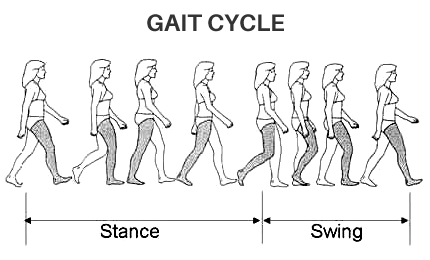
\includegraphics[width=0.65\textwidth]{chapter2/images/gaitcycle.png}
	\caption{วัฏจักรการเดินของมนุษย์}
	\label{fig:human_gait_cycle}
\end{figure}
\begin{enumerate}[label=\arabic*., leftmargin=1.5cm]
	\item ช่วงเริ่มการวางเท้าเพื่อเข้าสู่ช่วงเริ่มต้นเหวี่ยงเท้า เป็นช่วงที่เท้าเกิดการกระแทกลงบนพื้นหลังจากทำการเหวี่ยงมาจากด้านหลัง
	      โดยธรรมชาติมนุษย์จะทำการวางส้นเท้าลงเพื่อลดแรงกระแทกที่เกิดขึ้นในช่วงนี้
	      ดังนั้นทางกายภาพในส่วนของส้นเท้ามนุษย์จึงมีลักษณะอ่อนนุ่ม
	\item ช่วงเริ่มต้นเหวี่ยงเท้าเพื่อเข้าสู่ช่วงเหวี่ยงเท้า หลังจากทำการวางส้นเท้าลงกับพื้นแล้ว ข้อเข้าจะปรับมุมเพื่อให้ฝ่าเท้าแนบพื้นสนิท
	      ขณะเดียวกันขาอีกข้างจะยกสูงขึ้นเพื่อถ่ายเทน้ำหนักไปยังเท้าที่เพิ่งวางลง
	\item ช่วงเหวี่ยงเท้า เป็นช่วงที่ขาหนึ่งยกลอยอยู่ในอากาศและขาที่วางแนบกับพื้นจะรองรับน้ำหนักทั้งหมดของร่างกาย
	\item ช่วงเตรียมการวางเท้า เป็นช่วงที่ขาข้างที่ลอยอยู่เหวี่ยงไปข้างหน้าเพื่อเตรียมเข้าสู่ช่วงรองรับ 
	      ในขณะเดียวกันขาที่รับน้ำหนักอยู่จะทำการผลักตัวเพื่อเริ่มทำการถ่ายเทน้ำหนักไปข้างหน้า
\end{enumerate}

\clearpage
\subsubsection{การวิเคราะห์องศาอิสระของมนุษย์}
การที่มนุษย์สามารถเคลื่อนที่ได้เป็นผลเนื่องมาจากการเคลื่อนที่ของข้อต่อต่างๆ ซึ่งประกอบไปด้วย ข้อต่อส่วนสะโพก ส่วนหัวเข่า และส่วนข้อเท้า
แรงบิดที่เกิดขึ้นของแต่ละข้อต่อมีความสัมพันธ์ต่อกัน ส่งผลให้เกิดเสถียรภาพในการเดินของมนุษย์
เมื่อวิเคราะห์ลักษณะโครงสร้างในแต่ละส่วน พบว่าข้อต่อส่วนสะโพกมีลักษณะเป็นทรงกลม 
ทำให้ข้อต่อส่วนสะโพกสามารถหมุนได้ 3 องศาอิสระ ส่วนหัวเข่าของมนุษย์มีจุดต่อของข้อที่มีลักษณะเป็นทรงกลม
สองลูกประกอบเข้าด้วยกันทำให้การเคลื่อนที่ถูกบังคับให้สามารถเคลื่อนที่ได้เพียง 1 องศาอิสระ
ในส่วนของข้อเท้ามีลักษณะการเคลื่อนที่เหมือนสะโพกคือสามารถเคลื่อนที่ได้ 3 องศาอิสระ

จากทั้งหมดที่ได้ทำการวิเคราะห์มาข้างต้นพบว่าในขาหนึ่งข้างของมนุษย์ประกอบด้วย 7 องศาอิสระ
ซึ่งส่งผลให้การเคลื่อนที่ของมนุษย์มีความคล่องแคล่วสูง แต่ในทางออกแบบกลไกการเดินและการควบคุม
ของหุ่นยนต์สองขาถือว่ามีจำนวนองศาอิสระเกินความจำเป็นในการเคลื่อนที่บนปริภูมิ (space) และยากต่อการควบคุม
(underactuated) ดังนั้นการกำหนดจำนวนองศาอิสระเพื่อให้หุ่นยนต์เดินได้เสมือนมนุษย์จึงมีผลในการออกแบบกลไกทางกลและการควบคุมของหุ่นยนต์สองขา 

\begin{table}[!ht]
	\centering
	\begin{tabular}{|c|c|c|c|}
		\hline
		{ข้อต่อ}&{องศาอิสระ}&\multicolumn{2}{c|}{องศาการหมุน}\\
		\cline{3-4}
		{}                                     & {}         & {สูงสุด} & {ต่ำสุด} \\
		\hline
		\multirow{3}{*}{หัว}             & $\theta_x$ & +60                  & -30                  \\
		\cline{3-4}
		                                       & $\theta_y$ & +70                  & -70                  \\
		\cline{3-4}
		                                       & $\theta_z$ & +80                  & -80                  \\
		\hline
		\multirow{3}{*}{หลัง}          & $\theta_x$ & +30                  & -30                  \\
		\cline{3-4}
		                                       & $\theta_y$ & +55                  & -55                  \\
		\cline{3-4}
		                                       & $\theta_z$ & +45                  & -45                  \\
		\hline
		\multirow{3}{*}{หัวไหล่} & $\theta_x$ & +180                 & -80                  \\
		\cline{3-4}
		                                       & $\theta_y$ & +45                  & -135                 \\
		\cline{3-4}
		                                       & $\theta_z$ & +30                  & 0                    \\
		\hline
		{ศอก}                            & $\theta_x$ & 0                    & -155                 \\
		\hline
		\multirow{3}{*}{สะโพก}       & $\theta_x$ & +120                 & -40                  \\
		\cline{3-4}
		                                       & $\theta_y$ & +40                  & -50                  \\
		\cline{3-4}
		                                       & $\theta_z$ & +60                  & -50                  \\
		\hline
        {หัวเข่า}                & $\theta_x$ & 0                    & -130                 \\
        \hline
		\multirow{3}{*}{ข้อเท้า} & $\theta_x$ & +30                  & -60                  \\
		\cline{3-4}
		                                       & $\theta_y$ & +45                  & -20                  \\
		\cline{3-4}
		                                       & $\theta_z$ & +20                  & -60                  \\
		\hline
	\end{tabular}
	\caption{ความสามารถในการหมุนของแต่ละข้อต่อของมนุษย์}
	\label{tab:human_joint_limit}
\end{table}

ผู้เขียนได้ข้อสรุปในการออกแบบขาหนึ่งข้างของหุ่นยนต์ให้มีองศาอิสระเท่ากับ 6 องศาอิสระ และได้ใช้ดิจิตอลเซอร์โวของบริษัท Robotis เป็นตัวขับเคลื่อนข้อต่อ
เนื่องจากภายในเซอร์โวมีตัวรับรู้สถานะของตัวเอง และเซอร์โวนี้ถูกออกแบบมาให้สามารถติดตั้ง และสั่งการได้ง่าย

